\section{Experiments}\label{sec:experiments}
%%%%%%%%%%%%%%%%%%%%%%%%%%%%%%%%%%%%%%%%%%%

The proposed algorithm is part of a python package relying on numpy and numba~\parencite{harris2020,lam2015}.
It will be made open-source upon publication. To compare its efficiency, we used several public datasets described in \Cref{table:datasets}.
We performed an extensive benchmark with the following competitors:
\begin{itemize}[noitemsep]
  \item Alternating Direction Method of Multipliers (\texttt{admm})~\parencite{boyd2010}
  \item Anderson acceleration for proximal gradient descent (\texttt{anderson})~\parencite{zhang2020}
  \item Proximal Gradient Descent (\texttt{pgd})~\cite{combettes2005}
  \item Fast Iterative Shrinkage-Thresholding Algorithm (\texttt{fista})~\parencite{beck2009}
  \item Semismooth Newton-Based Augmented Lagrangian (\texttt{newt-alt})~\parencite{Ziyan2019}
  \item The Oracle solver (\texttt{oracle}) uses the clusters obtained via another
        solver to compute coordinate descent updates from the known solver.
  \item The Hybrid (ours) (\texttt{hybrid}) solver (see \Cref{alg:hybrid}) combines proximal gradient descent
        and coordinate descent to overcome the non-separability of the SLOPE problem.
\end{itemize}

\begin{table}[]
  \centering
  \label{table:datasets}
  \begin{tabular}{
      l
      S[table-format=6.0,round-mode=off]
      S[table-format=7.0,round-mode=off]
      S[table-format=1.4,round-mode=off]
      c
    }
    \toprule
    Datasets    & \(n\) & \(p\)   & {Density} \\ \midrule
    Simulated 1 & 200   & 20000   & 1         \\
    Simulated 2 & 20000 & 200     & 1         \\
    Simulated 3 & 200   & 2000000 & 0.001     \\ \hline
    Rhee2006  & 842   & 361     & 0.025        \\
    bcTCGA    & 536   & 17322   & 1         \\
    rcv1 & 20242   & 19959   & ?\\
    news20 & 19996 & 1355191 & ?  \\ \bottomrule
  \end{tabular}
\end{table}

We used the \texttt{benchopt}~\parencite{moreau2022benchopt} tool to obtain the convergence curves for the different solvers.
\texttt{Benchopt} launches each solver several times increasing the number of iterations and store the objective value, dual gap and time to reach it.
The repository to reproduce the benchmark is available at XXX.
The datasets used for the experiments can be found in \Cref{table:datasets} and were downloaded from \dataset{libsvm}\footnote{\url{https://www.csie.ntu.edu.tw/~cjlin/libsvmtools/datasets/}} and the university of Iowa webpage\footnote{\url{https://myweb.uiowa.edu/pbreheny/7600/s16/data.html}}.

\qk{Talk about how the sequence of $\lambda$ was chosen throughout the benchmarks}

\subsection{Simulated data}

The design matrix $X$ is simulated with correlation between features $j$ and $j'$ equal to $\rho^{|j-j'|}$ where $\rho$ is a parameter that can be chosen in $[0, 1[$.
The true regression vector $\beta^\star$ contains a certain number of non-zero entries that are obtained by simulating a gaussian distribution with zero mean and unit variance.
The observations are equal to $y=X\beta^\star + \varepsilon$ where $\varepsilon$ is a centered gaussian distribution with variance such that $\lVert X\beta^\star\rVert / \lVert \varepsilon \rVert = 3$.
\begin{figure*}[htb]
  \centering
  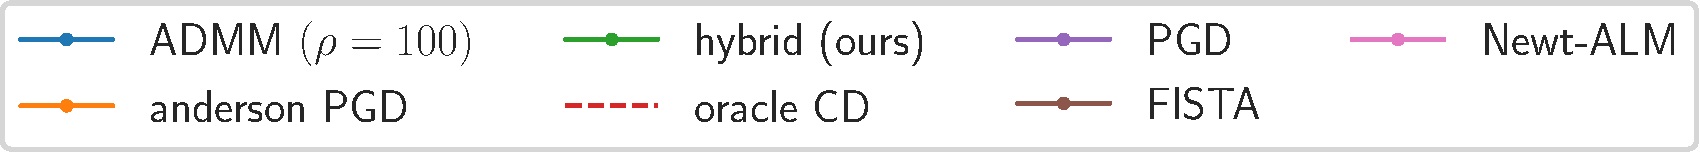
\includegraphics[scale=0.47]{simulated_legend.pdf}
  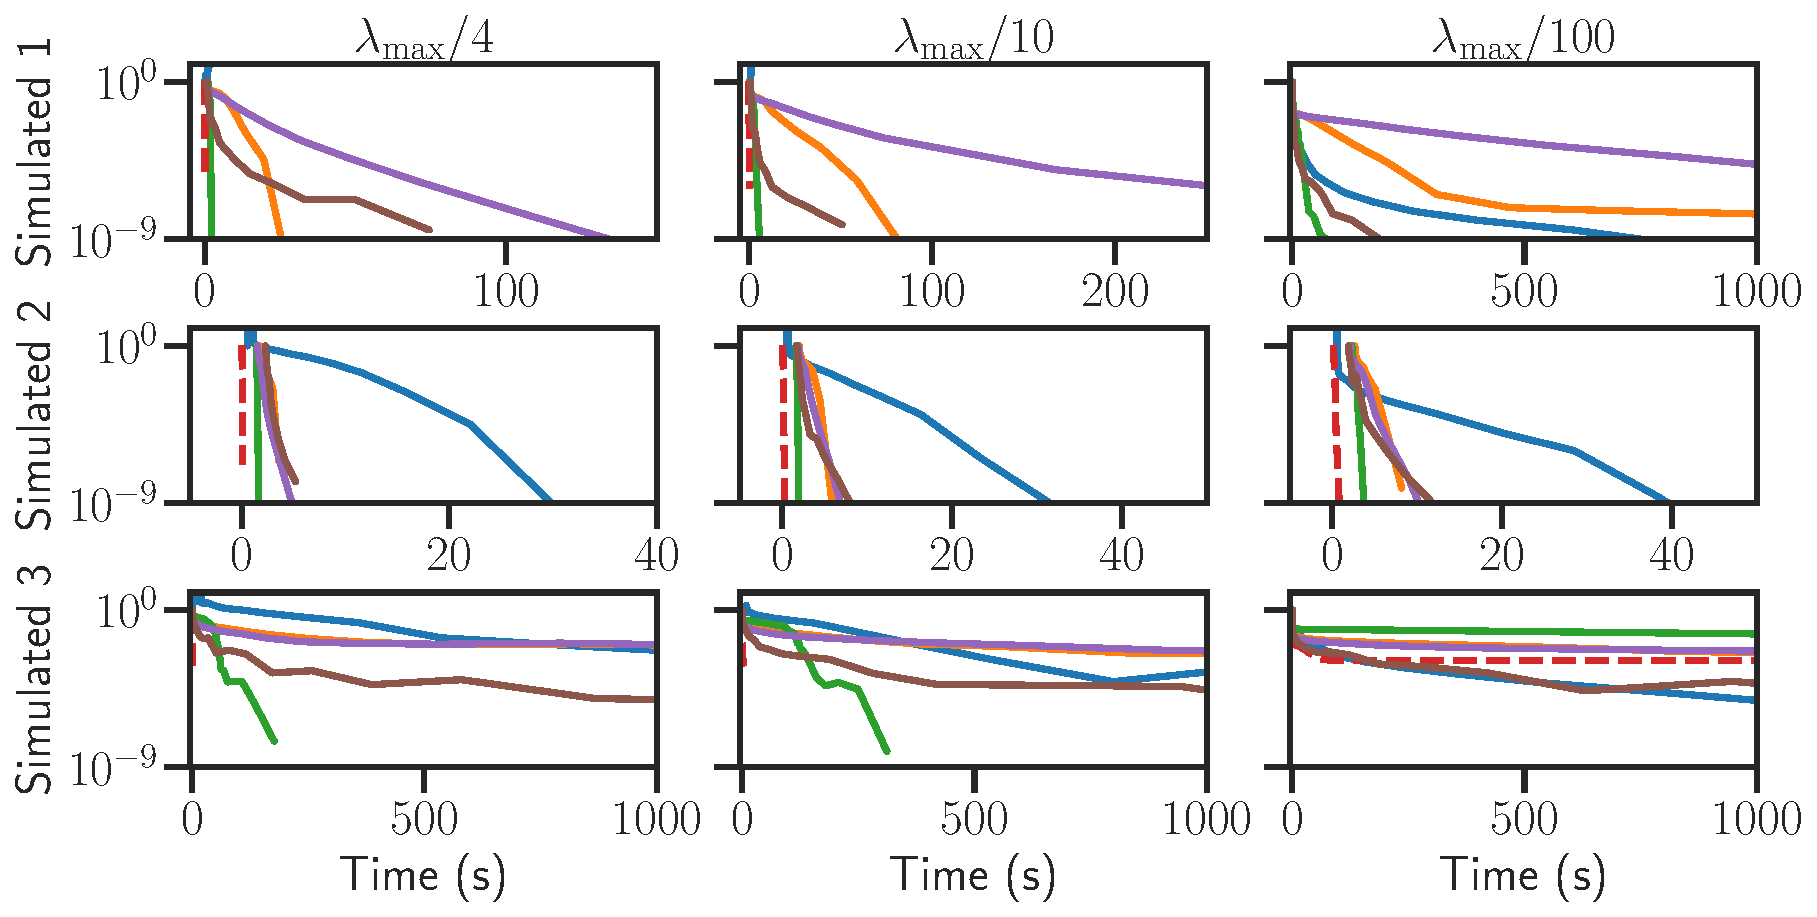
\includegraphics[scale=0.5]{simulated.pdf}
  \caption{\textbf{Benchmark on simulated datasets.} Normalized duality gap as a function of time for SLOPE on multiple simulated datasets and for multiple sequence of $\lambda$.}
  \label{fig:simulated}
\end{figure*}

In \Cref{fig:simulated}, we present the results of the benchmarks on simulated data.
The settings for the simulated can be found in \Cref{table:datasets}. 
We see that for smaller fractions of $\lambda_{\text{max}}$ our hybrid algorithm allows significant speedup in comparison to its competitors mainly when the number of features is large than the number of samples. 
On very large scale data such as in simulated data setting $3$, we see that the hybrid solver is faster than its competitors by one or two orders of magnitude. 


\subsection{Real data}
\begin{figure*}[htb]
  \centering
  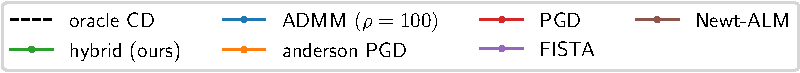
\includegraphics[scale=0.47]{real_legend.pdf}
  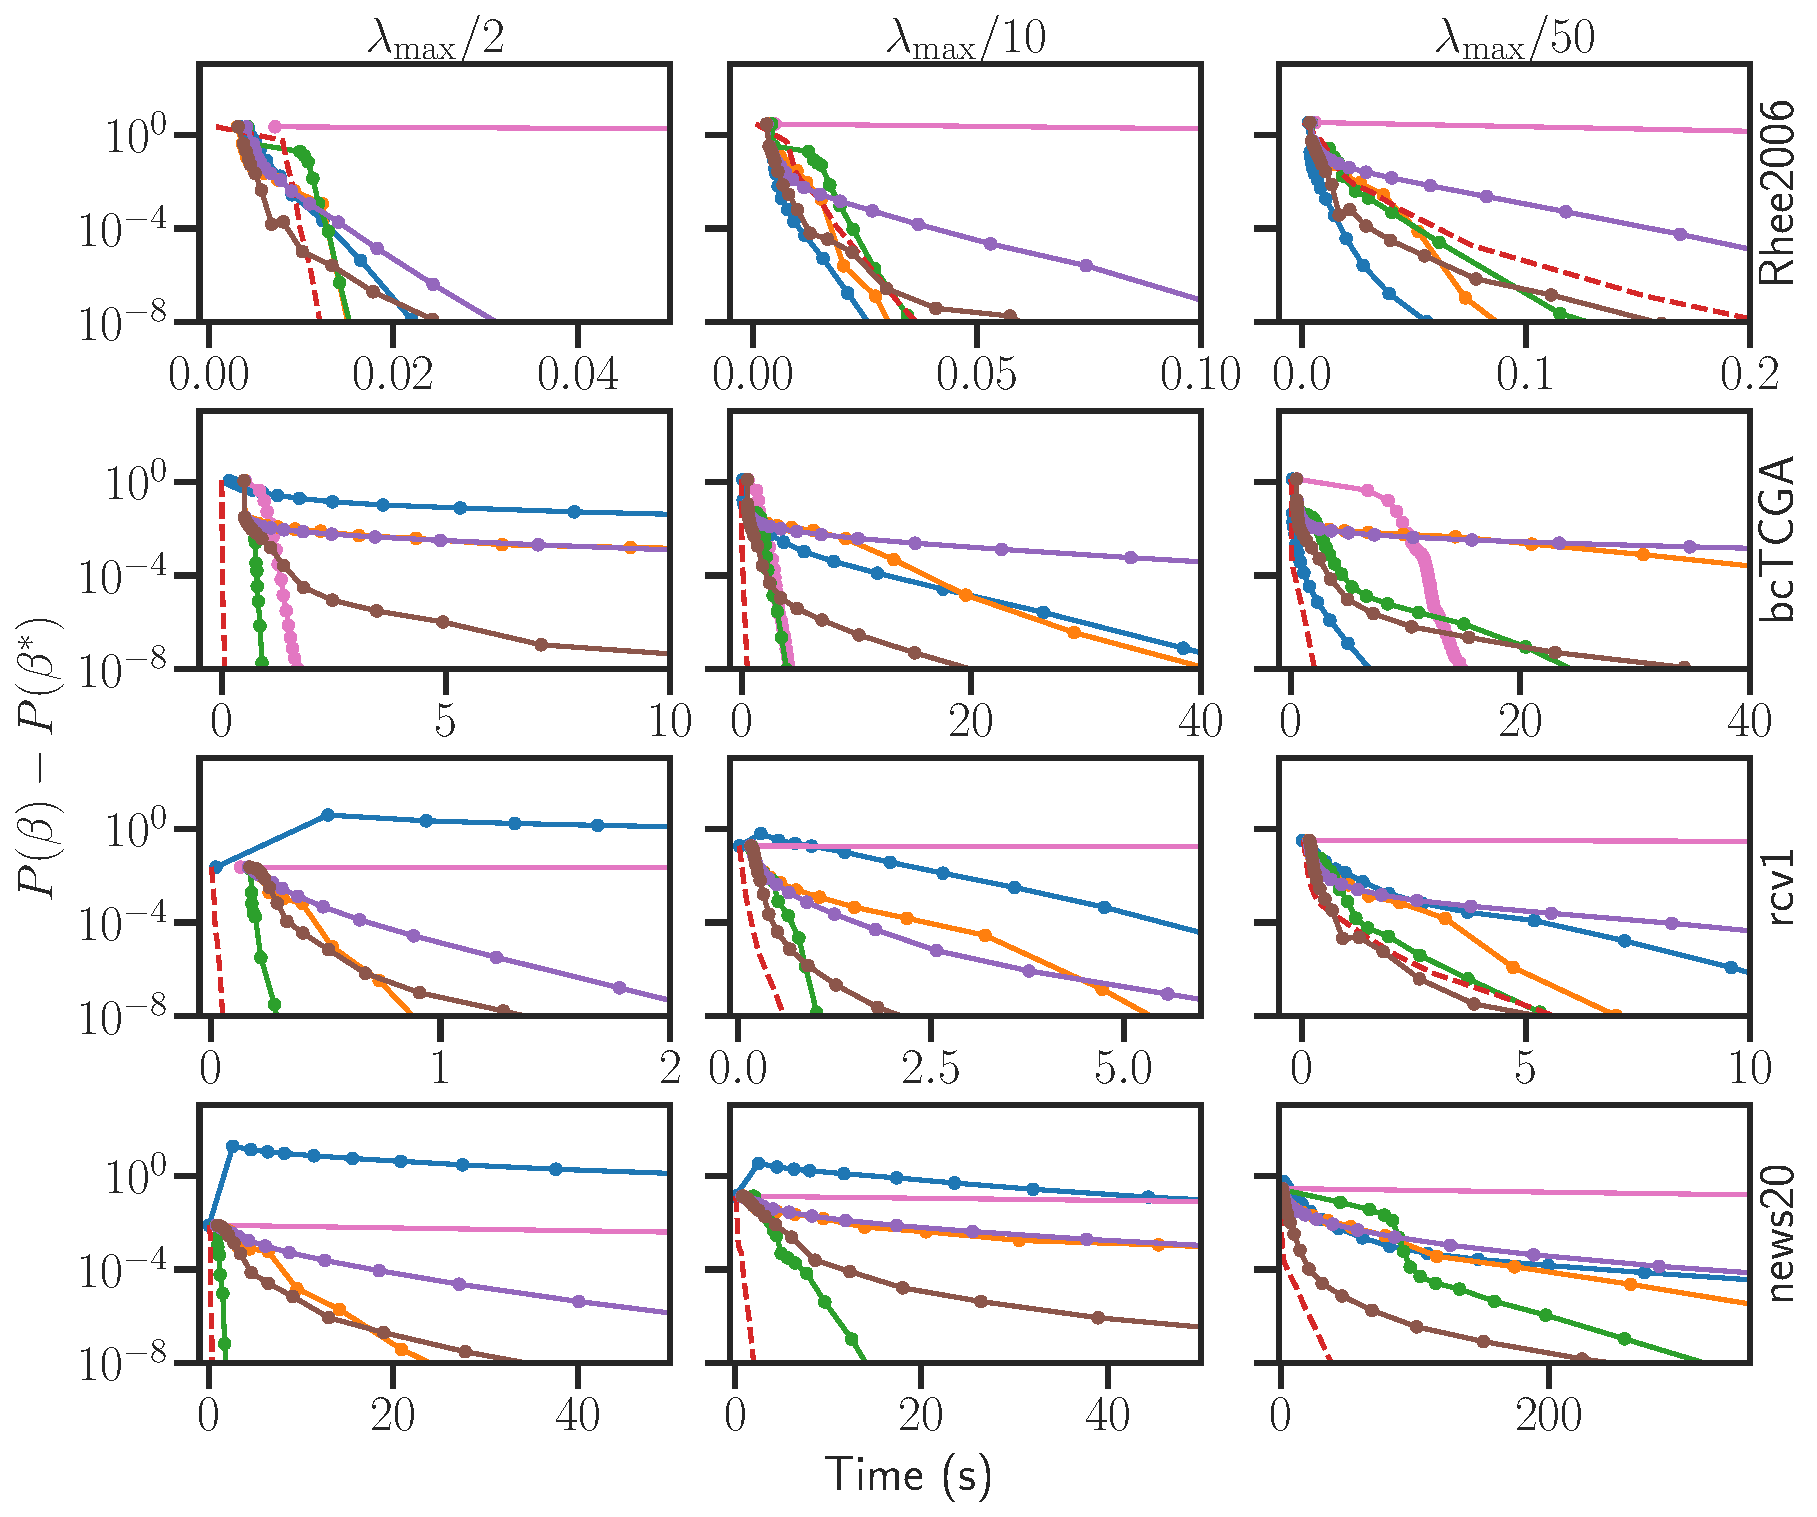
\includegraphics[scale=0.5]{real.pdf}
  \caption{\textbf{Benchmark on real datasets.} Normalized duality gap as a function of time for SLOPE on multiple simulated datasets and for multiple sequence of $\lambda$.}
  \label{fig:real}
\end{figure*}
